%! suppress = UnresolvedReference


\chapter{\app 的需求分析}\label{ch:req}


\section{应用面向的用户群体}\label{sec:target-user}

本应用的目标用户是佩戴可穿戴动态心电信号监测设备的院外患者。由于心血管疾病的发病率随着年龄增长而增加\cite{Zhongguoxinxieguanjiankangyujibingbaogao20212022},有动态心电监测需求的患者也以中老年人为主。除了常规的功能性需求分析之外,本项目也结合用户群体的特征进行了额外的非功能性需求分析以及相关的设计和实现。


\section{应用的功能性需求分析}\label{sec:func-req}

本应用的整体用例情况如图~\ref{fig:use-case} 所示。为了避免图像过于复杂,图中进行了一定程度的简化。

\begin{figure}[!ht]
    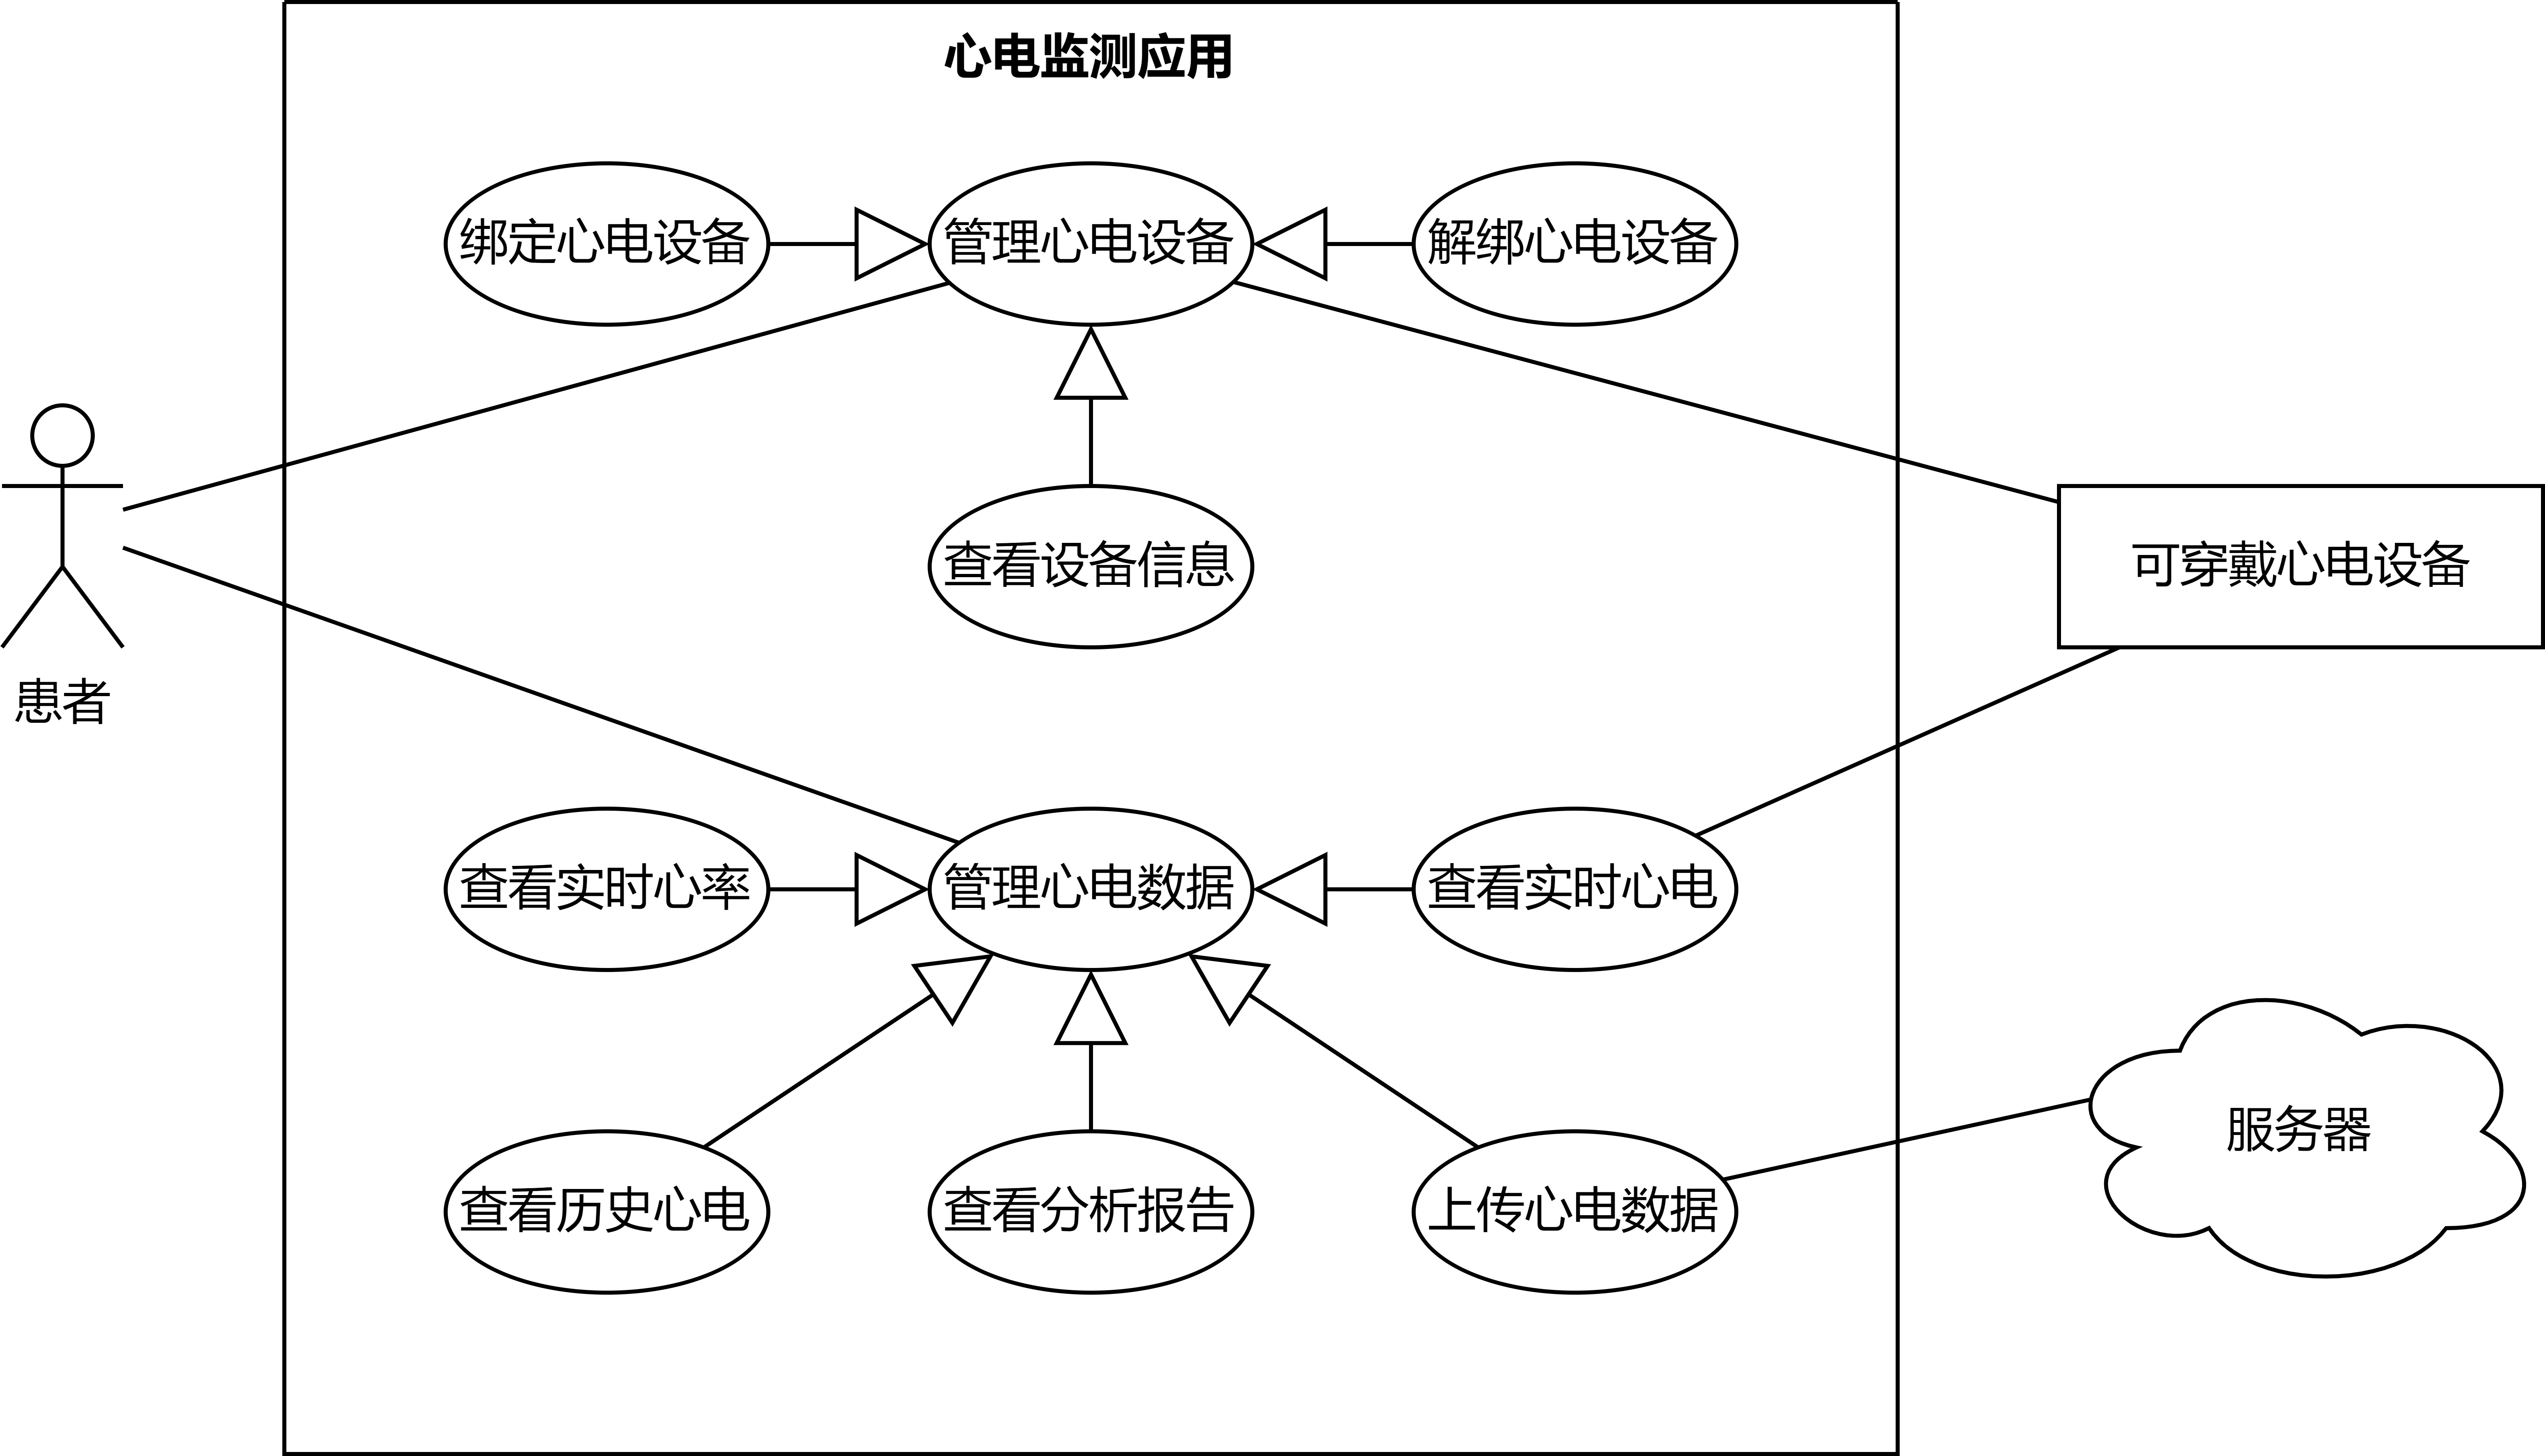
\includegraphics[width=\textwidth]{../assets/use-case.drawio}
    \bicaption{应用的用例图}{Use case diagram of the app}
    \label{fig:use-case}
\end{figure}

\subsection{心电设备相关需求分析}\label{subsec:device-req}

\subsubsection{绑定心电设备}

通常而言,新用户使用本应用的第一步是绑定其预先购买的动态心电信号监测设备(以下简称心电设备)。绑定心电设备的用例详情如表~\ref{tab:uc-bind-device} 所示。

\begin{table}[!ht]
    \centering
    \bicaption{绑定心电设备的用例详情}{Use case of binding a device}
    \label{tab:uc-bind-device}
    \begin{tabularx}{\textwidth}{|l|X|}
        \hline
        名称        & 绑定心电设备     \\
        \hline
        主要参与者     & 患者         \\
        \hline
        目标        & 绑定心电设备     \\
        \hline
        次要参与者     & 心电设备       \\
        \hline
        前置条件      & 未绑定心电设备    \\
        \hline
        后置条件(成功时) & 已绑定心电设备    \\
        \hline
        触发条件      & 患者尝试绑定心电设备 \\
        \hline
        主要事件流 &
        \begin{itemizec}
            \item[1.] 应用列出可绑定的心电设备,并定时刷新;
            \item[2.] 患者指定要绑定的心电设备;
            \item[3.] 应用绑定心电设备。
        \end{itemizec} \\
        \hline
        扩展事件流 &
        \begin{itemizec}
            \item[1a.] 没有可绑定的心电设备:应用提示用户没有可绑定的心电设备,并定时刷新。
        \end{itemizec} \\
        \hline
        异常事件流 &
        \begin{itemizec}
            \item[3a.] 绑定心电设备失败:应用提示用户绑定心电设备失败。
        \end{itemizec} \\
        \hline
    \end{tabularx}
\end{table}

\subsubsection{解绑心电设备}

用户在绑定心电设备后,可能会因为各种原因需要解绑心电设备。解绑心电设备的用例详情如表~\ref{tab:uc-unbind-device} 所示。

\begin{table}[!ht]
    \centering
    \bicaption{解绑心电设备的用例详情}{Use case of unbinding the device}
    \label{tab:uc-unbind-device}
    \begin{tabularx}{\textwidth}{|l|X|}
        \hline
        名称    & 解绑心电设备     \\
        \hline
        主要参与者 & 患者         \\
        \hline
        目标    & 解绑心电设备     \\
        \hline
        前置条件  & 已绑定心电设备    \\
        \hline
        后置条件  & 未绑定心电设备    \\
        \hline
        触发条件  & 患者尝试解绑心电设备 \\
        \hline
        主要事件流 &
        \begin{itemizec}
            \item[1.] 应用解除心电设备的绑定。
        \end{itemizec} \\
        \hline
    \end{tabularx}
\end{table}

解绑心电设备是应用程序单向的动作,不需要心电设备的参与或者同意,用户完全可以在心电设备已无法正常工作的情况下成功执行此用例。因此,该用例也没有异常事件流,应用保证其必定成功。


\section{应用的非功能性需求分析}\label{sec:nonfunc-req}

\subsection{应用的易用性需求分析}\label{subsec:usability}

因为大部分中老年的用户没有丰富的移动设备使用经验,所以设计一个简单直观、易于使用的应用程序很重要。界面设计应避免使用复杂的元素,以尽量简洁清晰为目标。

此外,由于一般患者通常不会具备专业的医学知识,所以应用程序内应该尽可能地避免使用过于晦涩难懂的专业术语。同时,对于应用内无法避免使用的部分术语应该提供明显且易于理解的解释,以便用户理解其含义。

\subsection{应用的无障碍需求分析}\label{subsec:accessibility}

应用需要考虑到用户在视力等方面的障碍,尽可能地保证用户能够在不同的环境下使用应用程序。例如,应用程序应该提供对大字号、粗体字、高对比度、深浅主题等内容的支持。

\subsection{应用的性能需求分析}\label{subsec:performance}

由于动态心电监测的需要,本应用会长期驻留在系统后台运行。因此,应用程序的性能对于用户体验至关重要。应用程序应该尽可能地保持较低的内存占用和较低的电量消耗,以保证用户的使用体验。

\subsection{应用的兼容性需求分析}\label{subsec:compatibility}

应用程序需要能够在各种主流移动设备上运行。这包括对于Android和iOS两大移动操作系统的支持,以及对于各种型号的移动设备的支持。在应用的设计与实现中,需要充分考虑到不同环境可以为应用提供的可用功能有所差别,以保证应用程序在不同环境下的兼容性。


\section{项目的可行性分析}\label{sec:feasibility}

\subsection{项目的技术可行性分析}\label{subsec:tech-feasibility}

本项目所需的技术主要包括移动应用开发和动态心电智能分析两大部分。关于移动应用开发,本项目预期使用Flutter框架,开发者此前已有相关的经验,具备技术可行性。关于心电智能分析,项目所属课题此前已有相关的算法成果\cite{songDongtaixindiantudezhinengjiancesuanfayanjiuyuyingyong2022},具备技术可行性。

\subsection{项目的经济可行性分析}\label{subsec:economic-feasibility}

本项目在经济方面的成本主要在于动态心电记录仪的获取。由于课题已与相关医疗公司达成合作,获取设备的成本较低,具备经济可行性。

\subsection{项目的法律与道德可行性}\label{subsec:legal-feasibility}

本项目在法律和道德方面的考量主要在于用于测试的心电数据的获取。由于互联网上可以找到许多经志愿者同意的公开的心电数据,因此本项目可以使用这些数据进行测试,具备法律和道德可行性。
